\documentclass[10pt]{article}
\usepackage{import}
\usepackage{tabularx}
\usepackage{listings}
\usepackage{qrcode}
\usepackage{tikz}
\usepackage{hyperref}
\usepackage{CJKutf8}
\usepackage{graphicx}
\usepackage{color, colortbl}
\usepackage[utf8]{inputenc}
\usepackage{amsmath}
\usepackage{amsfonts}
\usepackage{amssymb}
\usepackage{booktabs}
\usepackage{algorithm}
\usepackage{algpseudocode}
\usepackage{subcaption}
\usepackage[english]{babel}
\usepackage[export]{adjustbox}
\usepackage{enumerate}
\usepackage{lineno}
\usepackage{cite}
\usepackage{acronym}
\usepackage{geometry}
\usepackage{fancyhdr}
\usepackage{lipsum}
\usepackage{lastpage}
\usepackage{tgtermes}
\usepackage[usenames,dvipsnames]{xcolor}
\usepackage{tcolorbox}
\usepackage{tabularx}
\usepackage{array}
\usepackage{colortbl}
\usepackage{float}

\tcbuselibrary{skins}


\definecolor{unilogo}{HTML}{b3c5d0}
\definecolor{Gray}{gray}{0.9}
\geometry{a4paper, top=0.75in, bottom=1in, left=1in, right=1in}
\renewcommand{\baselinestretch}{1.5}

\newcounter{FAcounter}
\newcounter{NFAcounter}

\begin{document}
\thispagestyle{empty}
\pagenumbering{arabic}

\begin{titlepage}
	\begin{center}
		\begin{LARGE}
		\bf{Einzelprojekt 24/25 - Starfighter Alliance\\}
		\end{LARGE}
		\vspace{40pt}
		
		\vspace{15pt}
		\textbf{\Large Software-Projekt\\}
		\vspace{6pt}
		\textbf{\Large Universität Ulm}\\
		\vspace{6pt}
		\textbf{\Large Bachelor of Computer Science}\\
		\vspace{20pt}
		
		\textbf{\large
			Alhasan Ramadan\\
			Matrikelnummer: 1170485}
		\vspace{40pt}
		
		
\includegraphics[width=0.3\textwidth]{./1200px-Uni_Ulm_Logo_Ausschnitt.svg.png} \\[45pt]
		
		\vspace{35pt} % zusätzlicher Abstand
		\textbf{\Large Pflichtenheft}\\
		\textit{Unter Aufsicht von}\\
		\textbf{\large Aaron Molt}\\
		
		
		\vspace{40pt}
		
		
		\textbf{\large Institut für Softwaretechnik und Programmiersprachen, Ulm\\
			Prof. Dr. Matthias Tichy, Sabrina Böhm, Valentin Kolb\\
			Wintersemester 2024/25
		}\\
	\end{center}
% QR-Code in der rechten unteren Ecke mit Skalierung
\begin{tikzpicture}[remember picture, overlay]
    \node[anchor=south east, xshift=-1cm, yshift=1cm] at (current page.south east) {
        \scalebox{1.5}{ %Skalierungsfaktor
            \qrcode{https://gitlab.uni-ulm.de/softwaregrundprojekt/2024-2025/einzelprojekt/tutorium-aaron/ramadan-alhasan} %QR-Code 
      }
    };
\end{tikzpicture}
\end{titlepage}


\tableofcontents
\pagestyle{fancy}


\fancyhead[L]{Software-Projekt 24/25}
\fancyhead[C]{Pflichtenheft}
\fancyhead[R]{Universität Ulm}

\fancyfoot[L]{Alhasan Ramadan}
\fancyfoot[C]{\thepage/\pageref{LastPage}}
\fancyfoot[R]{v.2.1.5}

\renewcommand{\headrulewidth}{0.8pt} % Linie unter der Kopfzeile
\renewcommand{\footrulewidth}{0.8pt} % Linie über der Fußzeile

\hypersetup{colorlinks=false,urlcolor=uulm-in}

\title{Pflichtenheft - Starfighter Alliance}

\newcommand{\FA}[5]{
	\refstepcounter{FAcounter}
    \noindent
    \begin{tcolorbox}[
        colframe=unilogo,           % Rahmenfarbe
        colback=unilogo!10,         % Hintergrundfarbe der Box
        boxrule=0.5pt,              % Dicke des Außenrahmens
        left=2mm, right=2mm, top=1mm, bottom=1mm, % Innenabstand der Box
        rounded corners=all,        % Alle Ecken abrunden
    ]
        \begin{tabularx}{\textwidth}{l|X}
            \rowcolor{unilogo} \textbf{\textcolor{white}{ID}} & \textbf{\textcolor{white}{FA \theFAcounter}} \\
            \hline
            \textbf{TITEL:} & #1 \\
            \hline
            \textbf{BESCHREIBUNG:} & #2 \\
            \hline
            \textbf{BEGRÜNDUNG:} & #3 \\ 
            \hline
            \textbf{ABHÄNGIGKEITEN:} & #4 \\
            \hline
            \textbf{RISIKEN:} & #5 \\
        \end{tabularx}
    \end{tcolorbox}
    \vspace{15pt}\par
}


\newcommand{\game}{Starfighter Alliance}
%Hasan Ergänzung


\newcommand{\NFA}[6]{
	\refstepcounter{NFAcounter}
    \noindent
    \begin{tcolorbox}[
        colframe=unilogo,           
        colback=unilogo!10,        
        boxrule=0.5pt,              
        left=2mm, right=2mm, top=1mm, bottom=1mm, 
        rounded corners=all,        
    ]
        \begin{tabularx}{\textwidth}{l|X}
            \rowcolor{unilogo} \textbf{\textcolor{white}{ID}} & \textbf{\textcolor{white}{NFA \theNFAcounter}} \\
            \hline
            \textbf{TITEL:} & #1 \\
            \hline
            \textbf{BESCHREIBUNG:} & #2 \\
            \hline
            \textbf{BEGRÜNDUNG:} & #3 \\ 
            \hline
            \textbf{ABHÄNGIGKEITEN:} & #4 \\
            \hline
            \textbf{RISIKEN:} & #5 \\
        \end{tabularx}
    \end{tcolorbox}
    \vspace{15pt}\par
}

\newpage
    \section{Spielidee und Hintergrund}
Dieses Pflichtenheft fasst die Anforderungen an das Endlos-Flug-Spiel Starfighter Alliance zusammen, welches
in diesem Wintersemester (WiSe 24/25) als Einzelprojekt entwickelt werden soll.\\
\textit{"Die Rebellen-Allianz muss durch einen Meteoritengürtel fliegen, um vor der großen Macht des
Imperiums zu fliehen. Dabei stehen sich nun ein Starfighter und eine Horde an Meteoriten gegenüber.
Könnt ihr mehr Meteoriten ausweichen als ein Yedi oder endet ihr frühzeitig wie ein Stormtrooper?"}\footnotemark[1]\\
In diesem Dokument werden die genaue Funktionsweise sowie die Implementierungsrichtlinien
beschrieben.

\footnotetext[1]{Aus der Einleitung im \textcolor{blue}{\href{http://jerrymomoda.com/analysis-endless-runners/}{Lastenheft}}}

    \section{Einleitung}
Der Zweck dieses Dokuments ist es, eine detaillierte Beschreibung der Anforderungen, sowie der Benutzerschnittstelle für die Anwendung Starfighter Alliance bereitzustellen. Es wird abgegrenzt, welche Anforderungen erfüllt werden müssen, damit die entwickelte Anwendung vom Kunden akzeptiert wird. Im Folgenden wird auf die Systemfunktionalität und die Systemeinschränkungen, sowie Annahmen über das Produkt eingegangen. Zuletzt werden detaillierte Anforderungsspezifikation bereitgestellt.

    \section{Allgemeine Beschreibung}

    Starfighter Alliance ist ein Single-Player-Game aus dem Genre der Side-Scrolling Endless Runners.\\

\noindent \textit{"Ein Endless Runner ist ein Actionspiel, linear im Design ohne Ende, ohne Pausen oder Pausen, ohne Stufen oder wechselnde Levels. Es hat ein durchgehendes Level. Das Spiel beginnt langsam und leicht. Schauplätze sind unter anderem Wege, Straßen und Eisenbahnschienen. Mit zunehmender Geschwindigkeit des Spiels scheint der Spielercharakter immer schneller und schneller zu laufen, als wäre er auf einem riesigen Laufband. Hindernisse nähern sich immer schneller und schneller, was immer schnellere Reaktionen erfordert (...).  Der Spieler erliegt der Intensität und das Spiel ist vorbei. Ironischerweise werden sie „endlos“ genannt, denn für Spieler sind sie alles andere als das. Für die meisten kommt das Ende viel zu früh}.\footnotemark[2]\\

\noindent Es nimmt genau ein Spieler / eine Spielerin an einer Spielpartie teil. Ziel des Spiels ist es, mit dem Raumschiff im Weltall möglichst viele Wellen an Meteroiten zu überstehen.

\footnotetext[2]{Übersetzt aus \textcolor{blue}{\href{https://moodle.uni-ulm.de/mod/folder/view.php?id=833521}{jerrymomoda.com}}}

\newpage

\subsection{Ansichten}

Die Anwendung besteht aus mehreren Ansichten, sogenannten Screens, über welche Spielende mit dem Programm interagieren können.

    \begin{tcolorbox}[
        colframe=unilogo,           % Rahmenfarbe
        colback=unilogo!10,         % Hintergrundfarbe der Box
        boxrule=0.5pt,              % Dicke des Außenrahmens
        left=2mm, right=2mm, top=1mm, bottom=1mm, % Innenabstand der Box
        rounded corners=all,        % Alle Ecken abrunden
    ]
        \begin{tabularx}{\textwidth}{l|X}
            \rowcolor{unilogo} \textbf{\textcolor{white}{SCREENS}} & \textbf{\textcolor{white}{BESCHREIBUNG}} \\
            \hline
            \textbf{Start-Screen} & Nach dem Start der Anwendung befindet sich der Spieler / die Spielerin im Start-Screen. Die Ansicht bietet Buttons zum Starten des Spiels, Laden einer Konfigurationsdatei und Beenden des Spiels. Zusätzlich werden die Logos der genutzten Programme angezeigt, die anklickbar sind und zur jeweiligen Website führen. Die aktuelle Version des Spiels wird ebenfalls sichtbar dargestellt. \\
            \hline
            \textbf{Selection-Screen} & Der Spaceship Screen ermöglicht es den Spielenden, ein Raumschiff auszuwählen. Eine Liste verfügbarer Raumschiffe wird angezeigt, jedes mit einem Vorschaubild sowie den Eigenschaften Geschwindigkeit und Schusskraft. Durch Anklicken eines Raumschiffs wird zum Game Screen gewechselt. \\
            \hline
            \textbf{Game-Screen} & Im Game-Screen wird das eigentliche Spiel dargestellt. Der Spieler / die Spielerin agiert hier, indem er das Raumschiff steuert und Hindernissen ausweicht. Der Weltraum, das Raumschiff und auftauchende Hindernisse sind sichtbar. Wichtige Informationen wie die Anzahl der überstandenen Wellen, gesammelte Punkte und verbleibende Leben werden stets angezeigt. Das Spiel kann mit einem Knopf über einen separaten Pause-Screen pausiert werden. \\ 
            \hline
            \textbf{Pause-Screen} & Der Pause-Screen zeigt einen verschwommenen Hintergrund und enthält mehrere Buttons: einen zum Schließen des Spiels, einen zum Beenden des Spiels und einen zum Fortsetzen des Spiels. Dieser Screen ermöglicht es den Spielenden, das Spiel zu pausieren und Einstellungen vorzunehmen.\\
            \hline
            \textbf{End-Screen} & Der End-Screen wird angezeigt, wenn das Spiel zu Ende ist. Er zeigt das Raumschiff, die Anzahl der überstandenen Wellen und die Punkteanzahl. Zudem werden die besten 10 Ergebnisse des Highscores angezeigt, der in einer separaten Datei gespeichert wird. Das aktuelle Ergebnis wird hervorgehoben, um anzuzeigen, ob der Spieler / die Spielerin unter den besten 10 liegt. Ein Button ermöglicht es, zum Start-Screen zurückzukehren, um das Spiel erneut zu spielen. \\
        \end{tabularx}
    \end{tcolorbox}
    
\subsection{Systemeinschränkungen und Abhängigkeiten}

Die Anwendung wird durch die Prozessor- und/oder Grafikleistung des Systems begrenzt, auf dem es läuft. Um die Anwendung zu entwickeln, werden die Sprachen GDScript (1) und C\# (2) verwendet und in den Versionen \texttt{v4.3.stable.mono.official[77dcf97d8]} (1) und \texttt{.NET 6.0 / C\# 10.0} (2) benötigt. Später soll die Anwendung als Binary für Windows, Linux oder MacOS ausgeliefert werden (das spezifische System wird in Absprache mit dem Tutor / der Tutorin entschieden).

    \section{Spezifische Anforderungen}

  	Dieser Abschnitt enthält eine vollständige und detaillierte Auflistung sämtlicher spezifischer Anforderungen, die an das System gestellt werden. In 		diesem Zusammenhang wird eine gründliche Beschreibung des Systems sowie seiner verschiedenen Funktionen und Merkmale präsentiert. Alle wesentlichen 		Anforderungen werden klar und präzise formuliert, um sicherzustellen, dass das System den festgelegten Standards entspricht und alle gewünschten 			Leistungs- und Funktionsanforderungen erfüllt. Zudem werden hier die Interaktionen zwischen den verschiedenen Systemkomponenten und deren jeweilige 		Aufgaben beschrieben, um die Systemarchitektur vollständig zu verstehen.

    \subsection{Funktionale Anforderungen}

    Im Folgenden werden alle Anforderungen, die die grundlegenden Aktionen des Softwaresystems spezifiziert.
    
    	\subsubsection{Rahmenbedingungen}
    
	\FA{Single-Player-Spiel}{Dem Spieler steht nur eine Einzelspieler-Option zur Verfügung}{Es legt fest, dass keine Mehrspieler-Option vorhanden 			sein wird, und schränkt somit die Funktionen der Interaktion ein.}{NFA1, NFA3}{-}
	
	\FA{Konfiguration}{In der Start-Ansicht soll eine JSON-Datei als Konfigurationsdatei ausgelesen werden. In dieser Datei werden Eigenschaften wie Anzahl der Leben und Raumschiffwerte festgelegt.}{Die Konfigurationsdatei ermöglicht es, zentrale Spieleeinstellungen wie die Anzahl der Leben und Raumschiffwerte flexibel anzupassen, ohne den Code ändern zu müssen. Dies erleichtert zukünftige Anpassungen und eine benutzerfreundliche Steuerung der Spielparameter.}{JSON-Konfigurationsdatei}{Fehlerhafte oder unvollständige Datei kann zu falschen Spieleinstellungen führen.}
	
	\FA{Farben-Server}{Mit einem Client-Server-Modell wird vor Spielstart ein Server benutzt, um die Farbe des Raumschiffes festzulegen. Auf Anfrage an den Server wählt der Server zufällig eine von neun Farben aus und schickt diese dem Client zurück.}{Die Verwendung eines Client-Server-Modells zur Festlegung der Raumschiff-Farbe ermöglicht eine dynamische und zufällige Farbauswahl, die für jedes Spiel einzigartig ist. Dies trägt zur Individualisierung und Vielfalt des Spielerlebnisses bei.}{NFA2}{Verbindungsprobleme könnten dazu führen, dass keine Farbe zugewiesen wird.}
	
	\FA{Server-Antwort}{Im Falle einer erfolgreichen Anfrage des Clients ist der Antwort Code des Servers 200 und das data-Feld in der JSON-Datei enthält einen String mit der gewünschten Farbe. Falls die Anfrage fehlgeschlagen ist, ist der Code 400 für illegale Anfrage und 500 im Falle eines
internen Fehlers im Server.}{Diese Antwortstruktur stellt sicher, dass der Client korrekt über den Status der Anfrage informiert wird.}{NFA2}{Fehlerhafte Statuscodes oder fehlende Antwort könnten den Spielfluss stören.}
	
	\FA{Soundeffekte}{Das Spiel wird für das Zerstören von Hindernissen und Schüsse bestimmte Soundeffekte abspielen.}{Die Soundeffekte sorgen für akustische Rückmeldungen bei wichtigen Ereignissen, wie dem Zerstören von Hindernissen und Schüssen. Sie verstärken das Spielerlebnis.}{NFA3}{-}

	\subsubsection{Weltraum}
	
	\FA{Weltraum als Spielumgebung}{Der Weltraum stellt den Hintergrund des Spiels dar. Das Raumschiff kann diesen nicht verlassen.}{Diese Anforderung beschreibt eine Einschränkung und Regelung der Spielumgebung, die das Verhalten des Raumschiffs definiert.}{-}{-}
	
    	\subsubsection{Raumschiff}

	\FA{Steuerung des Raumschiffes}{Das Raumschiff kann sich in alle Richtungen (links, rechts, hoch und runter) bewegen, jedoch nicht drehen. Die 			Steuerung erfolgt mittels der Pfeiltasten (oder W,A,S,D).}{Die Bewegung und Steuerung des Raumschiffes gilt als essentielle Spielmechanik und 				bestimmt direkt den Spielablauf.}{-}{Koordinierung in der Spielwelt}

	\FA{Tempo des Raumschiffes}{Das Raumschiff bewegt sich immer mit konstantem Tempo und stoppt, sobald keine Richtungstaste mehr betätigt wird. Die 	Bewegungsgeschwindigkeit des jeweiligen Raumschiff wird hierbei mit einbezogen werden.}{Diese Anforderung präzisiert das Verhalten der Steuerung. 			Somit gilt sie ebenfalls als grundlegende Mechanik zur Steuerung der Spieldynamik.}{FA15}{Feinabstimmung für Raumschiffe mit verschiedenen 				Werten}   

	\FA{Leben des Raumschiffes}{Das Raumschiff hat eine gewisse Anzahl an Leben. Die Leben werden bei Aufprall mit einem Hindernis einzeln 					nacheinander abgezogen.}{Die Reduzierung der Leben ist eine direkte Spielverhaltensfunktion, die eine Interaktion mit einem Hindernis beschreibt und 		das Überleben und die Herausforderung im Spiel bestimmt.}{FA28}{Komplexität bei der Implementierung der Kollisionslogik, Performance-Probleme bei der 			Berechnung von Kollisionen}

	\FA{Größe des Raumschiffes}{Das Raumschiff ist ein quadratisches Objekt, das im Weltraum bewegt werden muss. Die Größe
	des Raumschiffs muss dem Weltraum angepasst sein und sollte ca. 1/10 der Breite des Weltraumes
	betragen.}{Diese Anforderung beschreibt die Eigenschaften des Raumschiffs, einschließlich der Größe und Form. Sie hat direkten Einfluss auf die 			Darstellung des Raumschiffs im Spiel und die Hitbox hat essentiellen Wert für die Grundspielregeln.}{FA31, FA33}{-}

	\FA{Auswahl des Raumschiffes}{Dem Spieler steht vor Spielbeginn eine Auswahl aus einer Menge an verschiedener Raumschiffe zur Verfügung. Es muss mindestens eines der folgenden Raumschiffe eingebaut werden: Millenium Falke, Y-Sternenjäger, X-Sternenjäger.}{Diese Aussage beschreibt eine konkrete Funktion des Spiels, nämlich die Auswahl eines Raumschiffs. Es handelt sich um eine Interaktionsmöglichkeit des Spielers.}{FA15, FA36}{-}
	
	\FA{Werte des Raumschiffes}{Die auswählbare Raumschiffe haben jeweils eine unterschiedliche Bewegungsgeschwindigkeit und eine unterschiedliche 			Schusskraft. Diese Werte sollen beim Auswählen der Raumschiffe dem Spieler / der Spielerin
	angezeigt werden.}{Die Anzeige dieser Werte beim Auswählen des Raumschiffs stellt sicher, dass der Spieler eine informierte Wahl treffen kann. Das 			betrifft die Spielmechanik und die Interaktion mit dem Spieler.}{FA23}{-}

    	\subsubsection{Schüsse}
    	
    	\FA{Abfeuern eines Schusses}{Der Spieler kann mit durch Drücken der Leertaste einen Schuss abfeuern.}{Dies ist eine direkte Steuerungsfunktion des Spiels.}{FA27}{-}
    	
    	\FA{Zerstörungskraft der Schüsse}
    	{Die abgefeuerten Schüsse des Spielers können Hindernisse durch Treffer zerstören.}
    	{Hier wird die spezifische Funktion der Schüsse beschrieben.}
    	{Der Trefferschaden hängt von der Schusskraft des jeweiligen Raumschiffes ab(FA15).}
    	{-}
    	
    	\FA
    	{Aufprallverhalten der Schüsse}
    	{Sobald ein Schuss ein Hindernis trifft, verliert das Hindernis eine bestimmte Anzahl an Leben, abhängig von der Schusskraft des ausgewählten Raumschiffes. Nach einem Aufprall löst sich der Schuss auf.}
    	{Die Anforderung beschreibt die Interaktionsweise der Schüsse mit Hindernissen.}
    	{FA15, FA23, FA29}
    	{-}
    	
    	\FA{Bewegung der Schüsse}{Ein abgefeuerter Schuss fliegt vom oberen Rand des Raumschiffs mittig aus der Abschussstelle senkrecht nach oben bis er ein Hindernis trifft oder aus dem Bild verschwindet.}{Diese Anforderung beschreibt die Bewegungsfunktion der Schüsse.}{-}{-}
    	
    	\FA{Schussrate}{Der Spieler muss, sobald er einen Schuss abgegeben hat, einen Timer abwarten, um den nächsten Schuss abfeuern zu können.}{Die Schussrate ist eine einschränkende Eigenschaft, die sich direkt auf die Spieldynamik mit Hindernissen auswirkt.}{FA23}{-}
    	
    	\subsubsection{Hindernisse}
    	
    	\FA{Bewegung der Hindernisse}{Die Hindernisse haben eine bestimmte Geschwindigkeit, die über Zeit leicht ansteigt.}{Diese Anforderung präzisiert das Verhalten der Hindernisse. Somit gilt sie ebenfalls als grundlegende Mechanik zur Steuerung der Spieldynamik.}{FA31}{Fehlerhafte Geschwindigkeitsskalierung könnte zu unspielbaren Hindernisbewegungen führen.}
    	
    	\FA{Leben der Hindernisse}{Ein Hindernis hat eine Anzahl an Leben. Durch Schüsse können Hindernisse Leben verlieren und zerstört werden, sobald sie keine Leben mehr besitzen. Die Anzahl der Leben hängt dabei von der Größe des Hindernisses ab (größere Hindernisse haben mehr Leben).}{Die Funktionsweise der Leben der Hindernisse ist eine direkte Spielverhaltensfunktion, die eine Interaktion mit dem Spieler beschreibt und das Überleben und die Herausforderung im Spiel bestimmt. Sie gilt als eine weitere Kernmechanik.}{FA25, FA30}{-}

	\FA{Größe der Hindernisse}{Jedes Hindernis hat eine bestimmte Größe. Die Höhe und Breite der Hindernisse sind variable, jedoch ist die Höhe der Hindernisse pro Welle nicht unterschiedlich.}{Die konstante Höhe der Hindernisse pro Welle sorgt für Vorhersehbarkeit und Balancing, damit die Spieler sich besser auf die Herausforderungen einstellen können.}{FA31}{-}	
	
	\subsubsection{Wellen}
	
	\FA{Wellenverhalten}{Eine Welle bezeichnet das Erscheinen von Hindernissen auf einer Höhe, die sich gemeinsam mit der gleichen Geschwindigkeit senkrecht von oben nach unten bewegen.}{Dies beschreibt die Art und Weise, wie eine Welle generiert wird und beschreibt das Wellenverhalten.}{Synchronisiert die Hindernisbewegungen und hat direkten Einfluss auf die Spielumgebung und die Platzierungslogik der Wellen.}{Synchronisierungsfehler könnten Wellen unterschiedlich schnell erscheinen lassen.}
	
	\FA{Generation der Hindernisse in den Wellen}{Pro Welle wird eine beliebige Anzahl an Hindernissen generiert werden, solange mindestens die 1,5-fache breite des Raumschiffs als Weg für das Raumschiff irgendwo in der Welle frei bleibt. }{Diese Anforderung gilt als wichtige Einschränkung der Wellen und damit als Balancing-Methode.}{FA10, FA33}{-}
	
	\FA{Wellenabstand}{Zwischen zwei Hinderniswellen muss mindestens 3 mal die Höhe des Raumschiffs als Platz frei gelassen werden. Hindernisse, die am unteren Rand den Weltraum verlassen, werden automatisch zerstört und verschwinden.}{Diese Anforderung beeinflusst die Schwierigkeit des Spieles und verändert die Spieldynamik.}{Platzierung von Hindernissen}{Fehlerhafte Abstandseinstellung könnte zu Überlappungen oder unerwünschten Pausen zwischen Wellen führen.}
	
	\subsubsection{Spielablauf}

	\FA{Start-Ansicht}{Der Spieler soll nach dem Starten des Spiels einen Start-Screen als Erste Ansicht sehen. Hier soll der Spieler durch Buttons zwischen dem Starten des Spiels, Laden einer Konfigurationsdatei und Beenden des Spiels navigieren können.}{Diese Anforderung beschreibt die Erste Ansicht und dessen Navigationsfunktion.}{(FA28?)}{-}
	
	\FA{Auswahl-Ansicht}{Es soll eine Raumschiff-Auswahl-Ansicht existieren, die es dem Spieler ermöglicht, ein Raumschiff für das Spiel auszuwählen. Eine Liste von verfügbaren Raumschiffen wird angezeigt, jedes mit einem Vorschaubild, der Geschwindigkeitseigenschaft und Schusseigenschaft. Durch Anklicken des gewünschten Raumschiffs wird in die Spiel-Ansicht gewechselt.}{Diese Anforderung beschreibt die zweite Ansicht und dessen Auswahlsfunktion und die Funktion, Raumschiffe und dessen Werte abzubilden.}{FA24}{-}
	
	\FA{Spiel-Ansicht}{Es soll eine Spiel-Ansicht als Hauptspielbereich existieren. Dieser Screen gilt als Hauptspielbereich, wird nach der Auswahl-Ansicht angezeigt und enthält den Weltraum mit dem ausgewählten Raumschiff und Hindernis-Wellen. Während des Spiels werden die ganze Zeit Informationen über die Anzahl bestandener Wellen, gesammelte Punkte und die derzeitigen Leben des Raumschiffes angezeigt werden. Das Raumschiff wird am unteren Bildschirmrand mittig positioniert. Bei Drücken eines Startknopfes beginnt ein sichtbarer Countdown, der von 3 auf 0 herunterzählt. Nach Ablauf des Countdowns ertönt ein Startsignal, das entweder als Ton oder durch den Text „Start“ angezeigt wird. Nach dem Startsignal kann das Raumschiff gesteuert werden und die Hinderniswellen beginnen. Ein Zähler, der die Anzahl der Wellen anzeigt, sowie eine Punkteanzeige werden am Bildschirmrand sichtbar sein. Wenn eine Welle von Hindernissen den unteren Bildschirmrand erreicht, erhöhen sich die Punkte. Wenn eine Welle komplett zerstört wurde gibt es mehr Punkte.}{Diese Anforderung beschreibt den Hauptspielbereich, in dem alle wichtigen Elemente des Spiels – das Raumschiff, Hindernisse und Statusinformationen – dargestellt werden. Die Anzeige von Statusinformationen wie Punkte, Leben und Wellenzahl gehört zu den Kernmechaniken des Spiels, da sie dem Spieler Rückmeldung über seine Fortschritte und seinen Zustand im Spiel gibt.}{FA25}{-}
	
	\FA{Spiel-Pausierung}{Es soll dem Spieler möglich sein, über einen Button das Spiel zu pausieren. Dies wird über einen weiteren Screen/Popup erreicht. Zusätzlich wird hier eine Fortsetzungsmöglichkeit über einen Button eingesetzt.}{Diese Anforderung ermöglicht es dem Spieler, das Spiel temporär zu unterbrechen und später fortzusetzen. Die Funktion der Pausierung stellt eine Interaktionsmöglichkeit dar und verbessert die Benutzerfreundlichkeit, da der Spieler das Spielgeschehen jederzeit anhalten kann, um z. B. eine Pause einzulegen.}{FA26}{-}
	
	\FA{End-Ansicht}{Wenn das Spiel zu Ende ist, wechselt die Spiele-Ansicht zur End-Ansicht und der Spielende-Screen zeigt das Raumschiff, die Anzahl der Wellen und die Punkteanzahl an. Zusätzlich zeigt er die besten 10 Ergebnisse des eigenen Highscores an. Das Ergebnis des jeweiligen Spiellaufs wird hier hervorgehoben. Es existiert ein Button, mit dem der Spieler nach Ende zurück zur Anfangs-Ansicht geleitet wird.}{Diese Anforderung beschreibt die Ansicht nach dem Ende des Spiels, in der die Spielergebnisse und der Highscore angezeigt werden. Die Anzeige der besten 10 Ergebnisse sowie der aktuellen Leistung des Spielers ist eine wichtige Funktion zur Motivation und bietet dem Spieler eine Rückmeldung über seine Erfolge. Diese Darstellung gehört zur Funktionalität des Spiels, da sie den Abschluss des Spiels und die Bewertung des Spielergebnisses umfasst.}{FA26, FA27}{-}
	
	\FA{Highscore}{Die 10 besten Ergebnisse des Highscores eines Spielers werden in einer extra Datei gespeichert. Dazu sollen mindestens die Anzahl an Wellen und die Punkte des aktuellen Spieldurchlaufs angezeigt werden.}{Dies beschreibt die Funktion einer Abspeicherung des Highscores. Die Speicherung der 10 besten Spielergebnisse ermöglicht eine kontinuierliche Verfolgung der besten Runs und fördert den Wettbewerb, indem die Daten dauerhaft erhalten bleiben.}{-}{Datenverlust bei fehlerhafter Speicherung.}

    	\subsubsection{Optional}

	\FA{Automatische Zielerfassung für Schüsse}{Das Spiel implementiert ein System zur automatischen Zielerfassung für Schüsse, sodass der Spieler auch bei motorischen Einschränkungen spielen kann.}{Diese Funktion ist wichtig für die Zugänglichkeit des Spiels und trägt dazu bei, dass das Spiel für ein breiteres Publikum spielbar bleibt.}{-}{Erhöhter Entwicklungsaufwand, um das Zielerfassungs- und Schusssystem genau zu justieren.}
	
	\FA{Farbeinstellungen für rot-grün Schwäche}{Das Spiel bietet eine Option, bei der die Farben für Spieler mit rot-grün Schwäche angepasst werden können.}{Diese Funktion ist wichtig, um das Spiel für alle zugänglich zu machen, insbesondere für Menschen mit Farbsehschwächen.}{-}{Falsche Kontrastwahl}
	
	\FA{Sprachauswahl}{Das Spiel bietet eine mindestens englische Sprachoption für alle Texte und Sprachausgaben.}{Die Möglichkeit, die Sprache zu wählen, stellt sicher, dass das Spiel für internationale Spieler zugänglich ist. Sie erleichtert es, das Spiel zu verstehen und zu genießen, und ist entscheidend für eine größere Reichweite des Spiels.}{-}{-}
	
	\FA{Schriftgrößenanpassung}{Das Spiel ermöglicht es, die Schriftgröße der Textanzeigen anzupassen.}{Die Anpassung der Schriftgröße sorgt dafür, dass Spieler mit eingeschränkter Sehkraft die Textinformationen problemlos lesen können.}{-}{Layout-Anpassung für verschiedene Bildschirmgrößen.}
	
	\FA{Code-Fenster}{In der Start-Ansicht gibt es ein Textfeld, wo man bestimmte Codes eingeben kann, um extra Inhalte freizuschalten.}{Diese Elemente tragen zur Dynamik des Spiels bei und fördern das Gefühl der Neugier.}{-}{Balancing}
	
	\FA{Dimension-Wechsel-Button}{In der Start-Ansicht sollte es einen Button geben, der bei Druck die Dimension des Spiels verändert.}{Funktionsverhalten eines Knopfes.}{NFA8}{-}
	
	\FA{Untertitel-Textfeld}{Für die Untertitel wird ein Textfeld mit dem jeweilig gesprochenem Satz angezeigt.}{Funktionsweise eines Textes.}{NFA9}{-}

	\newpage
		
    \subsection{Nicht-funktionale Anforderungen}

    Dieser Abschnitt spezifiziert die nicht-funktionalen Anforderungen an das Softwaresystem. Nicht-funktionale Anforderungen beziehen sich auf die 			Umstände, unter denen die geforderte Funktionalität erbracht werden muss. Sie beschreiben die Art und Weise, wie etwas zu tun ist.\footnotemark[3]

\footnotetext[3]{Definition aus \textcolor{blue}{\href{https://www.ifi.uzh.ch/rerg/courses/archives/hs11/re-i/Kapitel_11_NFAnf.pdf}{Department of Informatics Uzh}} (Seite 3 f.)}

    	\subsubsection{Rahmenbedingungen}

	\NFA{Robustheit}{Die Anwendung darf nicht absturzen. Bei 100 Spielen darf maximal 1 Spiel aufgrund eines ¨
Fehlers abgebrochen werden.}{Dies soll dem Spieler / der Spielerin ein gutes Spielerlebnis offenbaren.}{-}{-}

	\NFA{Lokales Spiel}{Die Anforderung setzt fest, dass das Spiel auf einem einzelnen Gerät laufen wird}{Diese Anforderung beeinflusst die 					Betriebsumgebung und Systemanforderungen, wirft also den technischen Aspekt des Projektes auf}{-}{-}
	
	\NFA{Server-Anbindung}{Der Server ist unter der URL softwaregrund.pro/jekt/ws/color erreichbar und unterstützt Verbindungen über ws:// auf Port 80 und wss:// auf Port 443. Er arbeitet nach dem Websocket-Protokoll. Eine WebUI zum Testen des Servers ist unter https://softwaregrund.pro/jekt/ verfügbar.}{Die Angabe der Serververbindung stellt sicher, dass der Client korrekt mit dem Server kommunizieren kann und ermöglicht einen einfachen Zugang zum Testen.}{-}{-}

    	\subsubsection{Sprachen und Technologien}

	\NFA{Anwendung- und Implementierungssprache}{Die Anwendungssprache kann Deutsch oder Englisch sein. Die Implementierungssprache und 						Dokumentationssprache müssen auf Englisch sein.}{Dies bezieht sich auf die Sprachenstandards und Dokumentation, nicht auf die Funktionsweise des 			Spiels.}{-}{-}

	\NFA{Entwicklungsumgebung}{Das Spiel wird in Godot entwickelt, und für die Grafiken werden Blender und Figma verwendet.}{-}{Mögliche Kompatibilitätsprobleme zwischen den Tools.}{-}
	
	
	\NFA{Plattformkompatibilität}{Die Anwendung muss mindestens auf entweder Windows 10 bzw. 11, auf Linux oder MacOS laufen.}{Beschreibt unter einem 		technischen Aspekt die unterstützten Plattformen, ohne Auswirkungen auf das Spielverhalten zu haben.}{Kompatibilität mit NFA3, mögliche 						plattformspezifische Bibliotheken oder Systemanforderungen.}{Unterschiede bei der plattformübergreifenden Anpassung. Aufwand für neue Tests und 				Optimierungen.}
	
	\NFA{Benutzerfreundlichkeit}{Das Spiel muss eine intuitive Benutzeroberfläche bieten, die es Spielern ermöglicht, alle Funktionen ohne eine ausführliche Anleitung zu verstehen.}{Eine intuitive Benutzeroberfläche erleichtert den Spielern das Verständnis der Funktionen, sodass sie schnell und ohne Anleitung spielen können. Das verbessert die Benutzererfahrung.}{-}{-}

    	\subsubsection{Hindernis-Typ}
    	
    	\NFA{Typen von Hindernisse}{Die Hindernisse sollen als Meteoriten oder auch als andere Weltraumelemente dargestellt werden.}{Hier wird eine Funktion der Ästhetik beschrieben, die Eigenschaften der Hindernisse ändern sich nicht. Somit hat dies keinen Einfluss auf das atomare Spielerlebnis.}{-}{-}

    	\subsubsection{Optional}
    	
    	\NFA{3D-Modus}{Das Spiel kann alternativ in einem 3D-Modus oder in verschiedenen Perspektiven wie First-Person oder Third-Person gespielt werden.}{Der 3D-Modus und die Perspektiven sind eine Erweiterung des Spielerlebnisses, die nicht die grundlegende Funktionalität beeinflussen.}{Zusätzliche Ressourcen für die 3D-Entwicklung und -Optimierung.}{Höherer Entwicklungsaufwand und mögliche Performance-Probleme.}
    	
    	\NFA{Untertitel}{Das Spiel enthält Untertitel für alle gesprochene Texte. Verbessert die Zugänglichkeit für hörgeschädigte Spieler.}{Untertitel sind eine Zugänglichkeitsfunktion, die das Spielerlebnis verbessert, ohne die Hauptfunktionalität des Spiels zu ändern.}{-}{Entwicklungsaufwand für die Untertitel.}
    	
    	\NFA{Übergänge zwischen Screens im "PowerPoint-Style"}{Die Übergänge zwischen den verschiedenen Bildschirmen des Spiels sollen animiert und dynamisch wie in PowerPoint dargestellt werden.}{Diese Art von Animation betrifft lediglich die Benutzeroberfläche und ist daher eine nicht funktionale Anforderung, die das visuelle Erlebnis verbessert, ohne die Spielmechanik zu beeinflussen.}{-}{Zu viele Animationen können die Spielperformance beeinträchtigen.}
    	
    	\NFA{Charakterstimmen bei Schiffswahl}{Bestimmte Raumschiffe sollen beim Auswählen von Charakteren Sprachzeilen haben.}{Diese Funktion betrifft die Benutzeroberfläche und das Audio, was das Spielerlebnis erweitert, jedoch keine grundlegende Spielmechanik beeinflusst.}{FA5}{Höherer Aufwand für die Erstellung und Integration der Sprachaufnahmen.}
    	
    	\NFA{Umgebungs-Szenerie auswählbar}{Es können Umgebungen wie die Verfolgung von Jango Fett durch Obi-Wan gewählt werden.}{Diese Funktion verändert die Umgebung und die visuelle Gestaltung des Spiels, aber nicht die Kernspielmechanik.}{-}{Erhöhter Entwicklungsaufwand für neue Umgebungen.}
    	
    	\NFA{Kamerafolgung beim Start des Raumschiffs}{Zu Beginn des Spiels gibt es eine Kameraführung, die das Raumschiff kurz verfolgt.}{Diese Funktion betrifft die visuelle Darstellung und nicht die zugrundeliegende Spielmechanik.}{-}{Zusätzlicher Entwicklungsaufwand für die Kameraführung.}
    	
    	\NFA{Barrel Rolls}{Das Raumschiff kann Barrel Rolls (Kreisflüge) durchführen.}{Diese Funktion ist eine zusätzliche Gameplay-Möglichkeit, die die Kontrolle und das visuelle Erlebnis erweitert, jedoch keine grundlegenden Spielfunktionen betrifft.}{NFA8}{Schwierigkeit bei der Implementierung von Flugeffekten.}
    	
    	\NFA{Schäden beim Verlieren eines Lebens}{Das Raumschiff wird beschädigt und zeigt sichtbare Veränderungen wie brennende Stellen.}{Diese Funktion betrifft nur die visuelle Darstellung der Spielfigur und nicht die zugrunde liegende Spielmechanik.}{-}{Möglicherweise zusätzliche Performance-Anforderungen durch Schadensdarstellung.}
    	
    	\NFA{Geheimfunktionen in der Read.me}{Bestimmte Code-Funktionen, wie "Order 66" oder "Starkiller", sind nur in der Read.me des Spiels dokumentiert.}{Diese Funktionen sind optionale Spielmechaniken, die nicht die grundlegende Spielsteuerung betreffen, sondern lediglich zusätzliche Inhalte darstellen}{-}{Niemand findet die}
    	
    	
    	\newpage
    	\section{Systemstruktur}
    	Die Systemstruktur beschreibt die wesentlichen Komponenten und deren Interaktionen innerhalb des Spiels. In diesem Kapitel wird die Architektur des Spiels im Detail dargestellt, um einen Überblick über die verschiedenen Systembestandteile und ihre Zusammenarbeit zu geben. Es wird gezeigt, wie die einzelnen Module – von der Benutzeroberfläche bis hin zu den Spiellogiken – in ein funktionierendes System integriert werden. Dabei wird auf die Struktur und Organisation der Hauptkomponenten, sowie auf die Kommunikationsflüsse zwischen ihnen eingegangen.
    	
    	\subsection{Zustandsdiagramme}
    	In diesem Abschnitt werden die Zustandsdiagramme für Starfighter Alliance vorgestellt. Sie zeigen die verschiedenen Phasen des Spiels und die Übergänge zwischen den Zuständen. Eine detaillierte Beschreibung der Diagramme folgt.

\subsubsection{Screens}    	
Das Diagramm beginnt mit dem Starten der Anwendung, wodurch der erste Zustand, der Start-Screen, aktiviert wird. Dieser Zustand ist in die Unterzustände Start und Settings unterteilt. Im Start-Zustand erfolgt die Initialisierung der Tasten (Entry), und die Hauptfunktion wartet auf die Eingabe des Spielers (Do). Der Spieler hat drei Optionen: den Exit-Button drücken, um die Anwendung zu verlassen, den Settings-Button, um in den Settings-Zustand zu wechseln.
Im Settings-Zustand wird beim Eintritt die Initialisierung der Einstellungen vorgenommen (Entry), die Do-Funktion zeigt alle Optionen an, und beim Verlassen (Exit) werden die Eingaben des Spielers gespeichert. Der Spieler kann zurück zum Start-Zustand oder zum nächsten Zustand über den Start-Button wechseln.
Im Selection-Zustand werden alle Raumschiffe angezeigt (Entry: Show all spaceships), und die Do-Funktion wartet auf die Eingabe des Spielers. Drückt der Spieler den Back-Button, geht es zurück zum Start-Screen. Wählt der Spieler ein Raumschiff, wird die Konfiguration gespeichert (Exit: Save player config) und der Übergang zum Game-Screen erfolgt.
Im Game-Screen-Zustand startet der Countdown-Zustand (Entry: Start Timer), wartet auf den Timer (Do: Wait for timer) und spielt das Startgeräusch ab (Exit: Play start sound). Während des Countdowns gibt es zwei Optionen: Drückt der Spieler den Pause-Button, wechselt der Zustand in den Pause-Zustand (Entry: Initialize buttons, Do: Wait for player input), und nach Drücken des Back-Buttons geht es zurück zum Countdown, wenn dieser noch nicht abgelaufen ist. Ist der Countdown vorbei, geht es in den Run-Zustand. Sobald der Countdown abläuft, geht es automatisch in den Run-Zustand.
Im Run-Zustand sind vier Subzustände aktiv, die in den nächsten Kapiteln detailliert beschrieben werden. Die Do-Funktion zeigt die Spielstatistiken an (Show stats). Die Abbruchbedingungen für alle Subzustände sind der Pause-Button oder die Zerstörung des Raumschiffs, was zum End-Screen führt. Im End-Screen-Zustand wird der Punktestand gespeichert (Exit), und der Highscore wird angezeigt (Do). Der Spieler kann entweder den Restart-Button drücken, um zurück zum Selection-Screen zu wechseln, oder die Anwendung über den Exit-Button verlassen.\\
\begin{figure}
	\centering
	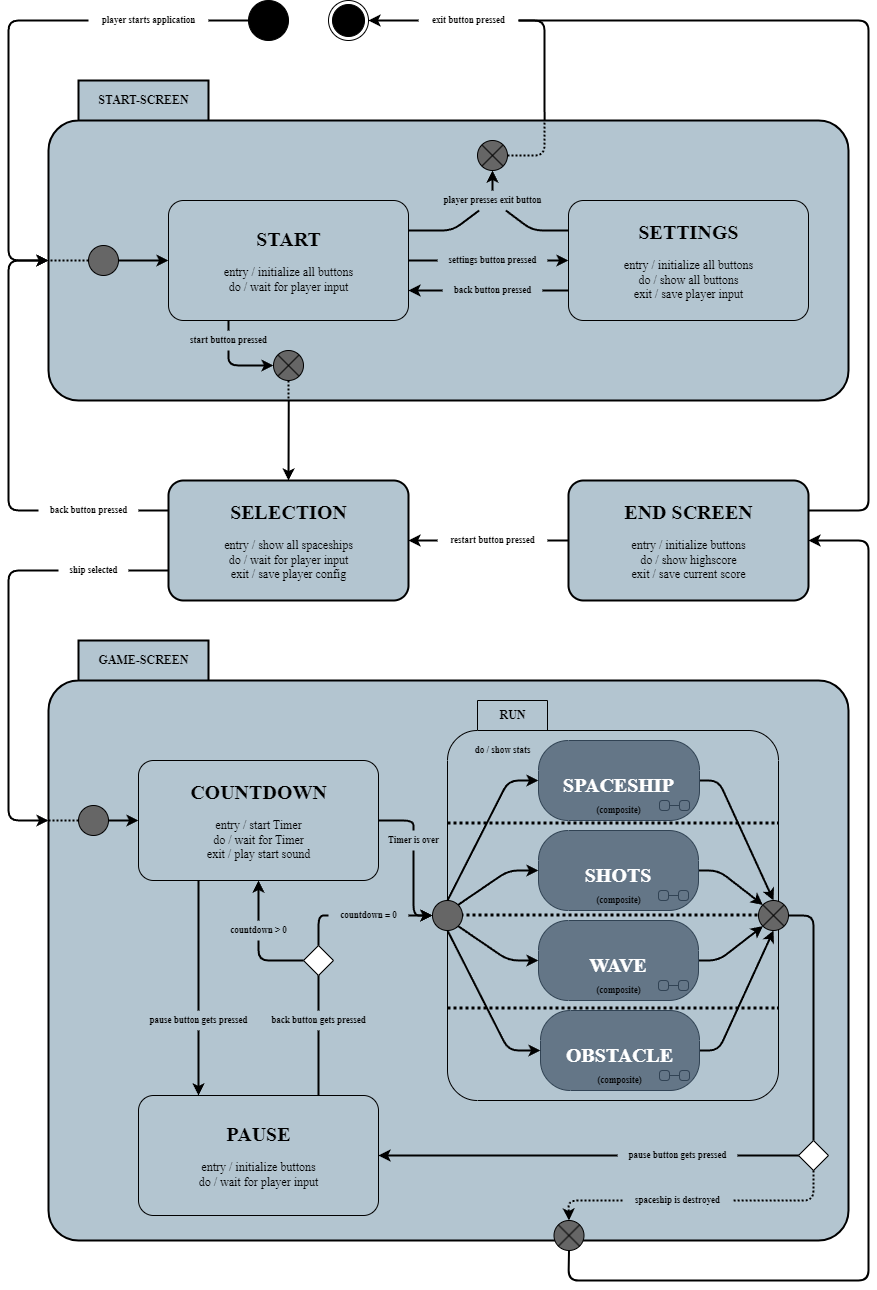
\includegraphics[width=1\textwidth]{../../../images/Pflichtenheft_Assets/uml-state-diagram/screens-state-diagram.png}\\
	\caption{screens-state-diagram.png}
\end{figure}

\newpage
\subsubsection{Spaceship}
Das Diagramm beschreibt die Zustände des Raumschiffs im Spiel.
Zu Beginn befindet sich das Raumschiff im Zustand Idle, welcher als Ruhemodus fungiert. Beim Eintritt (Entry) wird die Animation auf „Warten“ gesetzt, die Do-Funktion wartet auf eine Eingabe des Spielers, und beim Verlassen (Exit) wird die Bewegungsrichtung initialisiert. Solange keine Eingabe erfolgt, bleibt das Raumschiff im Idle-Zustand. Erfolgt jedoch ein Spielerinput (z. B. durch die Tasten W, A, S oder D), wechselt es in den Moving-Zustand.
Im Moving-Zustand wird beim Eintritt die Bewegungsanimation gestartet, die Do-Funktion sorgt für die kontinuierliche Bewegung des Raumschiffs, und beim Verlassen wird die Bewegung gestoppt. Hört der Spielerinput auf, wechselt das Raumschiff zurück in den Idle-Zustand.
Trifft das Raumschiff in einem der Zustände (Idle oder Moving) auf ein Hindernis, wird der Übergang abhängig von der verbleibenden Lebensanzahl gewählt. Sind die Leben auf 0 gesunken, wechselt das Raumschiff in den Destroyed-Zustand. In diesem Zustand wird beim Eintritt ein Zerstörungseffekt ausgelöst, die Do-Funktion zeigt eine visuelle Explosion, und beim Verlassen erfolgt der Übergang zum End-Screen.
Wenn noch Leben übrig sind, wechselt das Raumschiff in den Collision-Zustand. Beim Eintritt wird ein Leben abgezogen, die Do-Funktion aktiviert einen Unverwundbarkeitseffekt, und beim Verlassen endet dieser Effekt. Zur Sicherheit wird in diesem Zustand erneut geprüft, ob die Lebensanzahl tatsächlich nicht auf 0 gefallen ist. Nach Ablauf des Unverwundbarkeitseffekts kehrt das Raumschiff in den Idle-Zustand zurück.\\
\begin{figure}
	\centering
	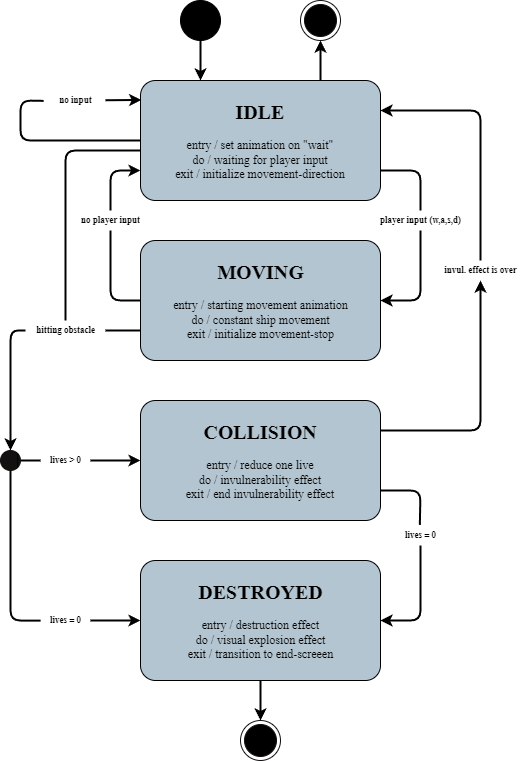
\includegraphics[width=0.55\textwidth]{../../../images/Pflichtenheft_Assets/uml-state-diagram/spaceship-state-diagram.png}\\
	\caption{spaceship-state-diagram.png}
\end{figure}

\newpage
\subsubsection{Shot}
Im Idle-Zustand wartet das System auf die Eingabe des Spielers (do: waiting for player input). Bei einem Tastendruck auf die Leertaste aktiviert sich die Schussmechanik, wodurch die Zustände Cooldown und Flight gleichzeitig eintreten.
Im Cooldown-Zustand startet ein Timer (entry: start Timer), und während der Laufzeit des Timers kann kein weiterer Schuss abgegeben werden (do: waiting for timer). Sobald der Timer abgelaufen ist, wechselt das System zurück in den Idle-Zustand.
Im Flight-Zustand wird die Bewegung des Schusses gestartet (entry: start moving animation) und währenddessen kontinuierlich fortgesetzt (do: constant shot movement). Verlässt der Schuss den Bildschirm, wird ebenfalls zum Idle-Zustand gewechselt. Trifft der Schuss jedoch ein Hindernis, erfolgt ein Wechsel in den Impact-Zustand mit einer Reduktion der Lebenspunkte des Hindernisses (entry: reduce obstacle life) und der Darstellung der Einschlag-Animation (do: impact animation). Nach Abschluss der Animation kehrt das System in den Idle-Zustand zurück.
\begin{figure}
	\centering
	\includegraphics[width=1\textwidth]{../../../images/Pflichtenheft_Assets/uml-state-diagram/shots-state-diagram.png}\\
	\caption{shots-state-diagram.png}
\end{figure}

\newpage
\subsubsection{Wave}
Wir beginnen im Idle-Zustand, der fortlaufend auf den Start einer neuen Welle prüft (do: check for new wave). Mit Beginn einer Welle wechselt das System in den Initialization-Zustand (entry: set starting positions der Hindernisse, abhängig vom Abstand) und startet die Erzeugung aller Hindernisse (do: initialize obstacles). Sobald alle Hindernisse bereit sind, wechselt das System in den Active-Zustand, wo die Hindernisbewegung eingeleitet wird (entry: start obstacle motion) und ein kontinuierlicher Abwärtsbewegungsprozess läuft (do: constant downward obstacle movement), wodurch die Welle aktiv dargestellt wird.
Falls das Raumschiff zerstört wird, kehrt das System in den Idle-Zustand zurück oder verlässt das Diagramm. Sobald alle Hindernisse den Bildschirm verlassen haben, wechselt das System in den Cooldown-Zustand, in dem ein Timer für die nächste Welle gestartet wird (entry: start timer for next wave, do: waiting for timer). Bei Ablauf des Timers wechselt das System zurück in den Idle-Zustand.
\begin{figure}
	\centering
	\includegraphics[width=0.7\textwidth]{../../../images/Pflichtenheft_Assets/uml-state-diagram/wave-state-diagram.png}\\
	\caption{wave-state-diagram.png}
\end{figure}

\newpage
\subsubsection{Obstacle}
Wenn eine Welle startet, beginnt das Hindernis im Moving-Zustand, in dem die Bewegungsanimation startet (Entry: starting movement animation) und die konstante Bewegung erfolgt (Do: constant obstacle movement).
Wird das Hindernis getroffen, gilt: Hat es keine Leben mehr, wechselt es in den Destroyed-Zustand mit Zerstörungseffekt (Entry: destruction effect), visueller Explosion (Do: visual explosion effect) und Übergang zum End-Screen beim Verlassen. Hat das Hindernis noch Leben, wechselt es in den Collision-Modus, in dem ein Leben abgezogen (Entry: reduce one life) und eine Aufprall-Animation gezeigt wird (Do: impact animation). Danach wird erneut geprüft: Ist das Leben auf 0, wechselt es in den Destroyed-Zustand, andernfalls kehrt es in den Moving-Zustand zurück.
Verlässt das Hindernis im Moving-Zustand den Bildschirm, erfolgt ebenfalls der Übergang in den Destroyed-Zustand.
\begin{figure}
	\centering
	\includegraphics[width=0.8\textwidth]{../../../images/Pflichtenheft_Assets/uml-state-diagram/obstacle-state-diagram.png}\\
	\caption{obstacle-state-diagram.png}
\end{figure}

\newpage
	\subsection{Klassendiagramm}

In diesem Abschnitt wird das Klassendiagramm\footnotemark[4] für Starfighter Alliance vorgestellt. Es zeigt die verschiedenen Klassen des Systems, deren Attribute und Methoden sowie die Beziehungen zwischen ihnen. Eine detaillierte Beschreibung des Diagramms nach Ansichten der Software-Architektur folgt.

\footnotetext[4]{Referenz aus \textcolor{blue}{\href{https://sparxsystems.com/resources/tutorials/uml2/class-diagram.html}{sparxsystems.com}}}

\begin{figure}
\centering
	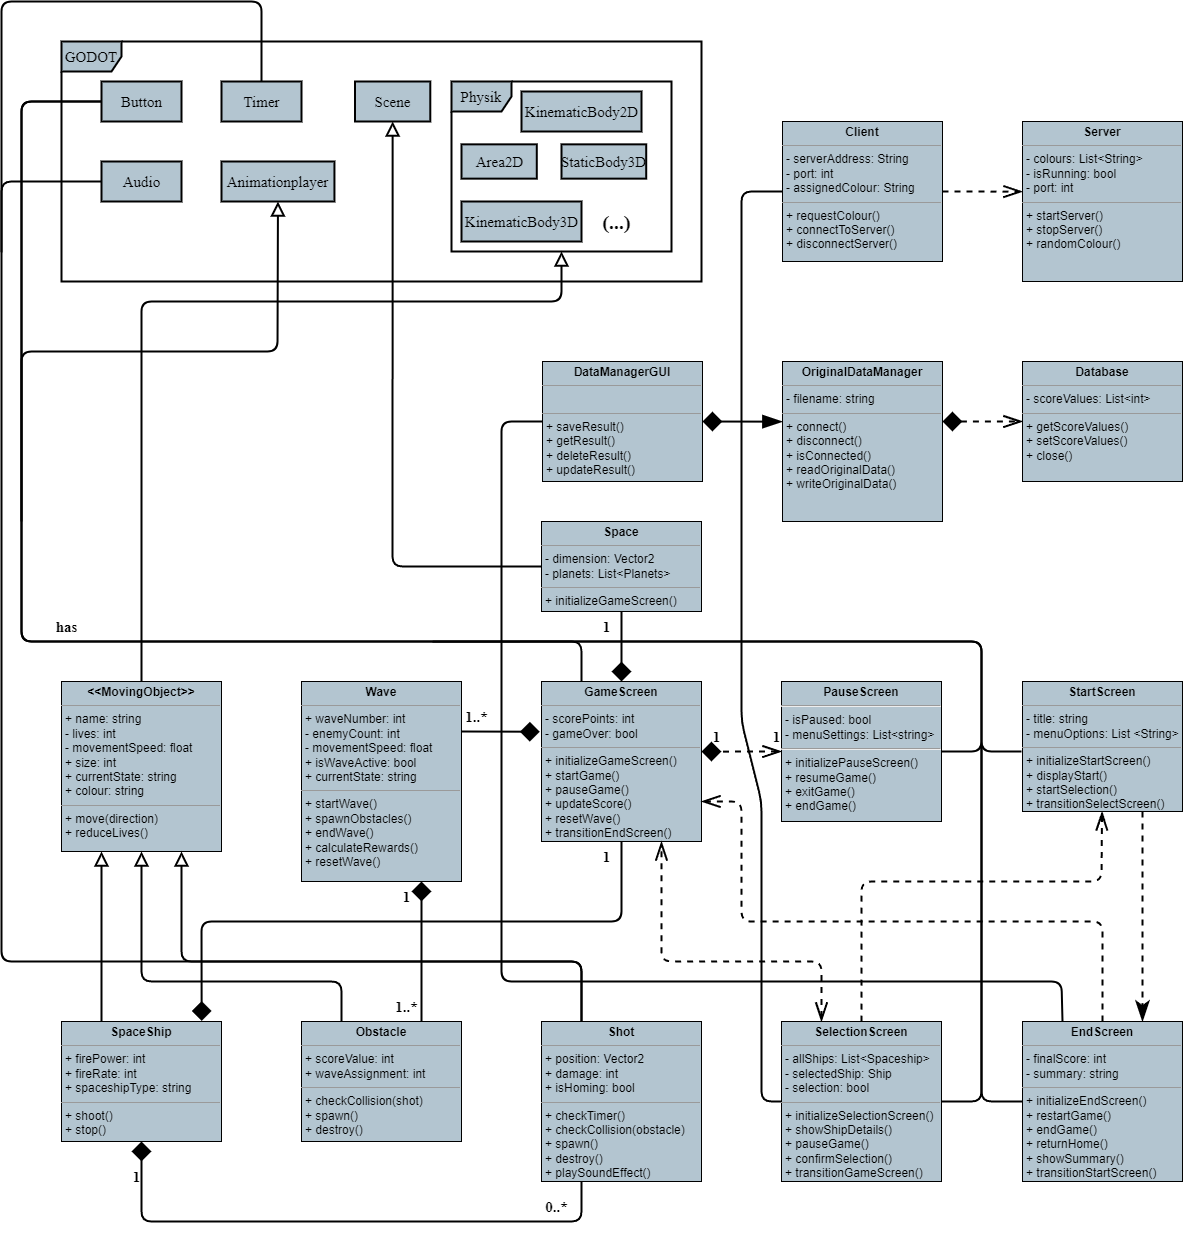
\includegraphics[width=1\textwidth]{../../../images/Pflichtenheft_Assets/uml-class-diagram/uml-class-diagram.png}\\
	\caption{uml-class-diagram.png}
\end{figure}
\newpage
\subsubsection{Logical View (Logische Sicht)}

Die logische Sicht beschreibt die statische Struktur des Systems, einschließlich der wichtigsten Klassen und deren Beziehungen:
\begin{itemize}
    \item \textbf{Hauptbildschirme des Spiels}: Die Klassen StartScreen, GameScreen, PauseScreen, EndScreen und SelectionScreen verwalten die verschiedenen Zustände des Spiels.
    \item \textbf{Datenmanagement-Komponenten}: Klassen wie DataManagerGUI, OriginalDataManager und Database kümmern sich um die Speicherung und Verwaltung von Highscores und Spieldaten.
    \item \textbf{Netzwerkkomponenten}: Die Klassen Client und Server ermöglichen Netzwerkfunktionen für den Multiplayer oder den Austausch von Daten.
    \item \textbf{Spielobjekte und Mechaniken}: Klassen wie SpaceShip, Wave, Obstacle und Shot modellieren die Spielfunktionalitäten. Die Basisklasse MovingObject fasst Eigenschaften und Methoden für bewegliche Objekte zusammen.
\end{itemize}

\subsubsection{Implementation View (Implementierungssicht)}

Die Implementierungssicht beschreibt die Organisation des Codes und die Verwendung von Bibliotheken und APIs:
\begin{itemize}
    \item \textbf{Datenmanagement und JSON-Verarbeitung}:
    \begin{itemize}
        \item Die Klasse ConfigurationManager liest eine JSON-Konfigurationsdatei ein, um zentrale Spieleinstellungen wie Raumschiffwerte und Leben bereitzustellen.
        \item DataManagerGUI und OriginalDataManager organisieren den Zugriff auf die Database\footnotemark[5] zur Speicherung von Highscores.
    \end{itemize}
    \item \textbf{Godot-API-Integration\footnotemark[6]}:
    \begin{itemize}
        \item Komponenten wie Button, Timer, AnimationPlayer und KinematicBody2D aus der Godot-Engine werden für Benutzerinteraktionen, Animationen, Bewegung und Physik genutzt.
    \end{itemize}
\end{itemize}

\footnotetext[5]{Aufbau der Datenklasse aus \textcolor{blue}{\href{https://www.researchgate.net/figure/Class-diagram-of-the-database-management-module_fig4_357706024}{researchgate.net}}}
\footnotetext[6]{GODOT Implementierung übernommen aus \textcolor{blue}{\href{https://docs.godotengine.org/en/stable/contributing/development/core_and_modules/godot_architecture_diagram.html}{docs.godotengine.org}}}


\newpage
\subsubsection{Process View (Prozesssicht)}
Die Prozesssicht beschreibt die dynamischen Abläufe und Interaktionen der Klassen während der Laufzeit:
\begin{itemize}
    \item \textbf{Spielsteuerung}:
     Die Klasse GameScreen verwaltet den Hauptspielablauf. Methoden wie startWave() und updateScore() steuern die Spiellogik.
    \item \textbf{Interaktionen zwischen Spielobjekten}: Objekte wie SpaceShip, Shot und Obstacle interagieren dynamisch, zum Beispiel durch Kollisionserkennung.
    \item \textbf{Datenoperationen}:
DataManagerGUI ruft Daten aus der Database ab oder speichert neue Einträge.
    \item \textbf{Netzwerkoperationen}:
Client und Server synchronisieren Daten über das Netzwerk.
\end{itemize}

\subsubsection{Deployment View (Verteilungssicht)}
Die Deployment-Sicht beschreibt die physikalische Verteilung der Software-Komponenten:
\begin{itemize}
    \item \textbf{Lokale Architektur}:
Das Spiel läuft auf einem Client-Gerät mit der Godot-Engine, die sowohl für Rendering als auch für die Spiellogik verantwortlich ist.
    \item \textbf{Netzwerkarchitektur}:
Der Server wird auf einer separaten Maschine oder in der Cloud betrieben, um Daten von mehreren Clients zu synchronisieren.
    \item \textbf{Datenhaltung}:
Die Database (zum Beispiel SQLite oder ein anderes lokales Speichersystem) speichert die Highscores auf dem Client oder Server.
\end{itemize}

\subsubsection{Benutzeroberfläche und Godot-Integration}

Das System nutzt verschiedene Komponenten der Godot-API für die Benutzeroberfläche und Spielfunktionen:

\begin{itemize}
    \item \textbf{Interaktive Elemente}: Button und Timer werden in den Bildschirmen (StartScreen, PauseScreen etc.) verwendet, um Benutzerinteraktionen zu steuern.

    \item \textbf{Audio und Animationen}: Die Komponenten Audio und AnimationPlayer werden genutzt, um Soundeffekte und Animationen abzuspielen.

    \item \textbf{Physik und Kollisionserkennung}: Komponenten wie KinematicBody2D und StaticBody2D ermöglichen Bewegung und Kollisionserkennung für Objekte wie SpaceShip, Shot und Obstacle.
\end{itemize}

\end{document}
